
% \documentclass[manuscript]{aastex}
\documentclass[12pt,preprint]{aastex}
%\documentclass[preprint2]{aastex}
%\documentclass[aaspp4]{aastex}
%\documentclass{aastex}
%\documentclass[]{emulateapj}
%\documentclass[onecolumn]{emulateapj}

%!TEX TS-program=latex
\usepackage{amsmath}
%\usepackage{pdfsync}
%\def\snp{SN\,II-P} 
%\def\snep{SNe\,II-P} 
%\def\VmI{\hbox{$V\!-\!I$}} 
%\def\fe{\ion{Fe}{2}}
%\newcommand{\bvri}{\protect\hbox{$BV\!RI$} }

\citestyle{aa}

\begin{document}

% \slugcomment{Draft \today}
%\submitted{Draft \today} 

\title {Ay 190 Worksheet 4} 
\shorttitle{WS4}
\shortauthors{Kleiser}

\author{Io Kleiser} \affil{Caltech} \email{ikleiser@caltech.edu}

\section{Description of the Network Code}

At the top of the code, several constants are defined as well as parameters for the EOS of a white dwarf (i.e. $\Gamma$ and $K$ in the polytrope euqation). Central and minimum densities are also defined here. The main routine is called tov\_integrate, which takes in the maximum radius for the grid and the number of zones. It calls set\_grid, which simply creates an array of radial zones which each have a thickness $dr$. tov\_integrate then defines the central pressure (based on the polytrope equation) and sets the central $M(r)$ to zero, then iterates outward through the zones. In this iteration, it first uses one of the Runge-Kutta methods (e.g. in tov\_RK2) to calculate values of pressure and interior mass for the $i+1$ zone. It also defines a surface at the minimum density above which the mass will not increase. Then it calculates the density and energy density based on the pressure. The outputs of this routine are: a $4\times n_z$ array (where $n_z$ is the number of zones) containing $\rho(r),~P(r),~\epsilon(r),$, and $M(r)$; the surface radius; and the width of the zones.

\section{First Convergence Test and Profile Plots}


\begin{figure}[!ht]
\begin{center}
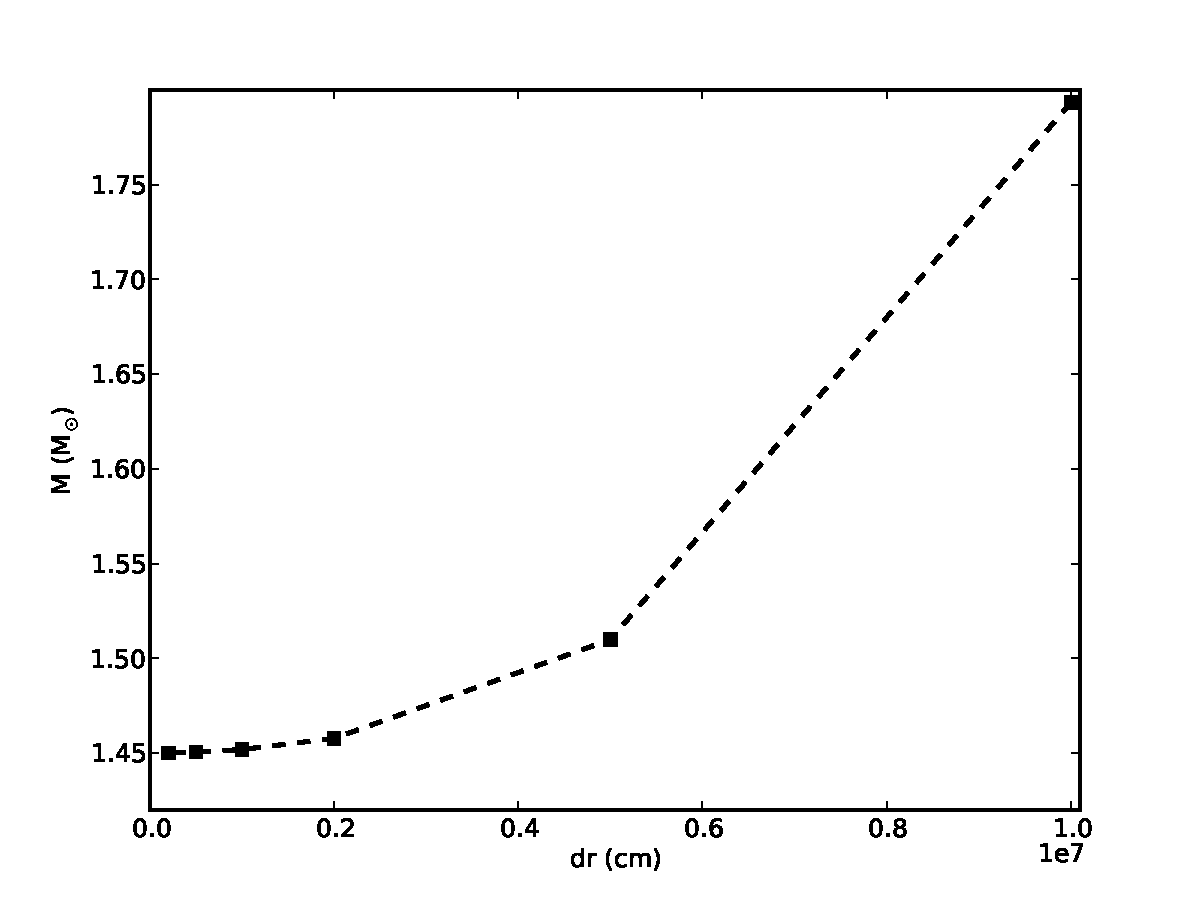
\includegraphics[width=5in]{RK2_mass.pdf}
\end{center}
\caption{Mass calculated by RK2 as a function of the zone size $dr$. The calculation converges on the correct value for high numbers of zones. The highest number of zones used is 5000. \label{f:RK2_mass}}
\end{figure}

\begin{figure}[!ht]
\begin{center}
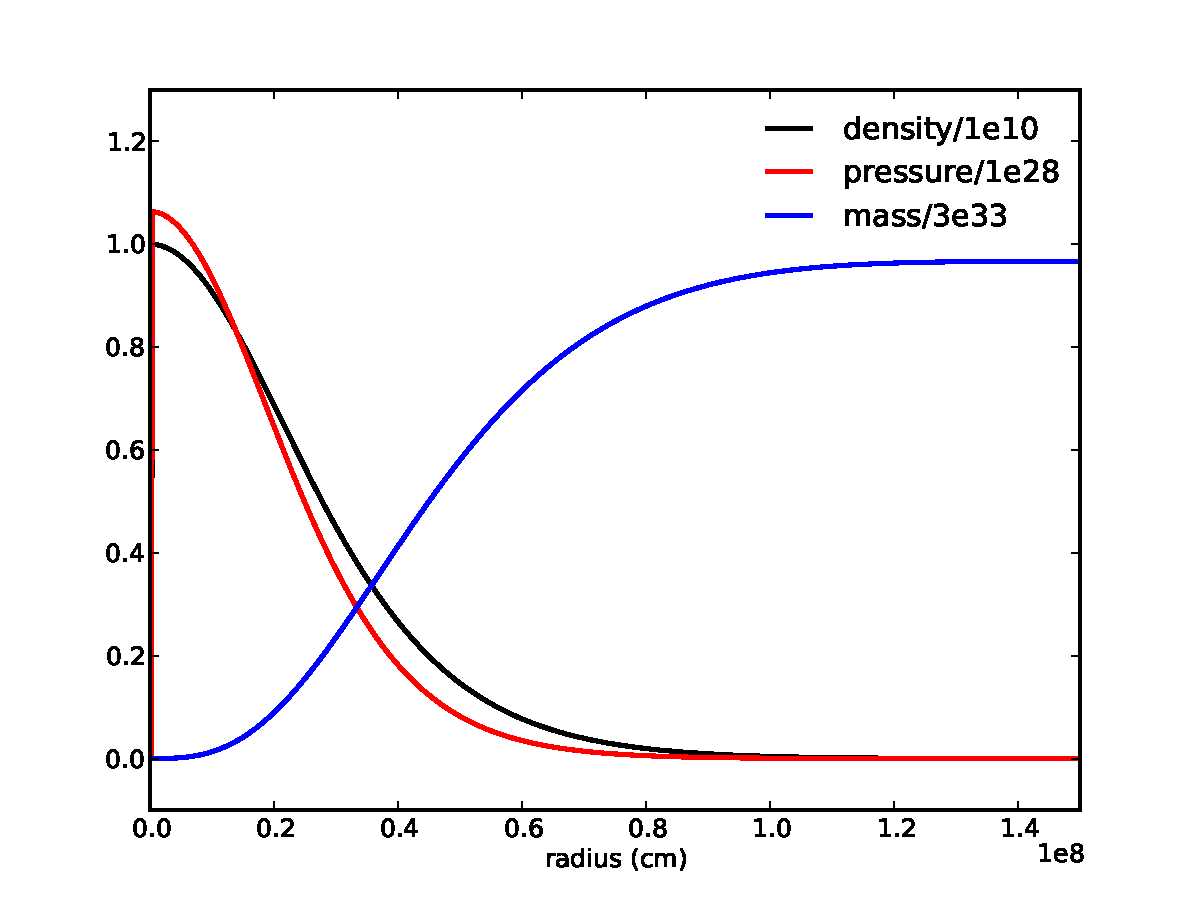
\includegraphics[width=5in]{profiles.pdf}
\end{center}
\caption{Density, pressure, and mass as a function of radius using 5000 zones and RK2. \label{f:profiles}}
\end{figure}

\begin{figure}[!ht]
\begin{center}
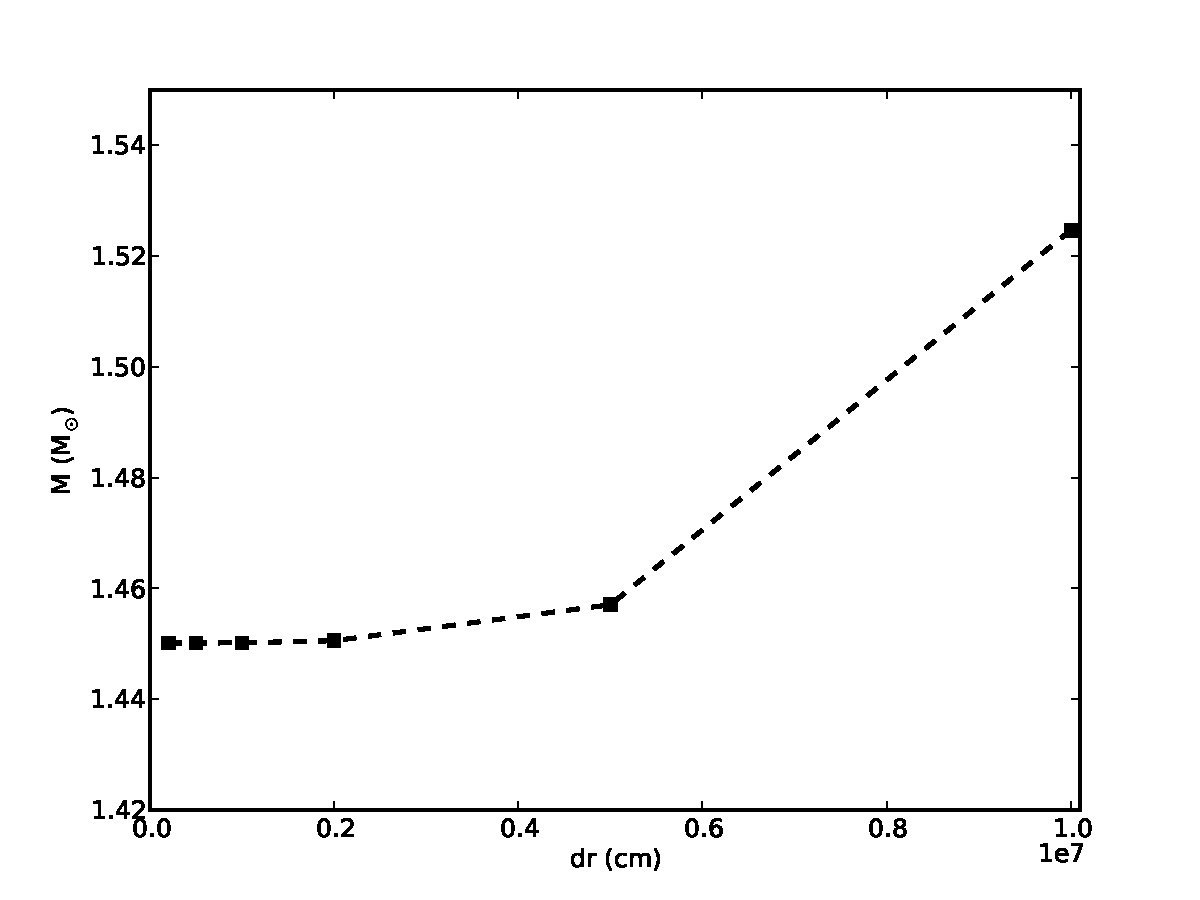
\includegraphics[width=5in]{RK3_mass.pdf}
\end{center}
\caption{ \label{f:RK3_mass}}
\end{figure}

\begin{figure}[!ht]
\begin{center}
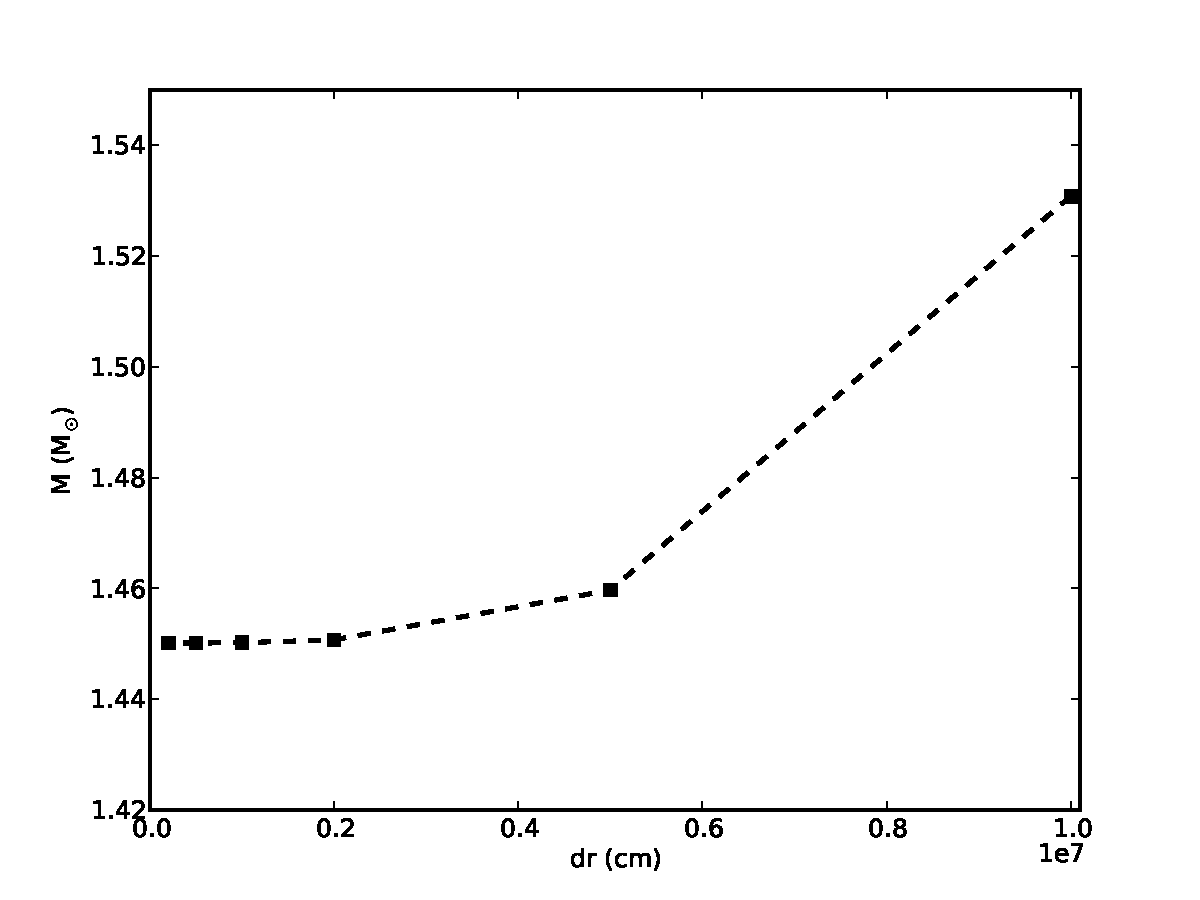
\includegraphics[width=5in]{RK4_mass.pdf}
\end{center}
\caption{ \label{f:RK4_mass}}
\end{figure}


%\bibliographystyle{apj2} 
%\bibliography{gal}

%\bibliography
\end{document}
